\documentclass[11pt]{article}
\usepackage[utf8]{inputenc}
\usepackage[T1]{fontenc}
\usepackage{amsmath,amssymb}
\usepackage{graphicx}
\usepackage{xcolor}
\usepackage{booktabs}
\usepackage[margin=2.2cm]{geometry}
\usepackage{array}
\usepackage{fancyhdr}

\definecolor{azul}{RGB}{0,70,140}
\definecolor{grisbox}{RGB}{245,247,250}

\newcommand{\seccion}[1]{%
  \vspace{4pt}\noindent{\color{azul}\large\bfseries #1}\par\vspace{2pt}\hrule\vspace{6pt}}

\pagestyle{fancy}\fancyhf{}
\rhead{\small Modelado y Simulación}
\lhead{\small Resolución de examen}
\cfoot{\thepage}

\setlength{\parindent}{0pt}
\setlength{\parskip}{4pt}

\begin{document}

\begin{center}
  {\color{azul}\LARGE\bfseries Resolución completa del examen}\\[2pt]
  {\large Sistemas dinámicos — Modelado y Simulación}\\[2pt]
  \rule{\textwidth}{0.8pt}
\end{center}

%==================================================================
\seccion{Ejercicio 1 — Sistema lineal 2D (punto silla)}

Sistema:
\[
\begin{cases} \dot{x}=x-2y\\[2pt] \dot{y}=-2x+y\end{cases}
\qquad\Longrightarrow\qquad
\dot{\vec{x}}=A\vec{x},\quad
A=\begin{pmatrix} 1 & -2\\ -2 & 1\end{pmatrix}.
\]

\textbf{Punto de equilibrio.} Se busca $\dot x=0,\ \dot y=0$. Como
\[
\det(A)=(1)(1)-(-2)(-2)=1-4=-3\neq0,
\]
el único equilibrio es el \textbf{origen} $(0,0)$.

\textbf{a) Nulclinas.}
\[
\dot x=0:\ x-2y=0\ \Rightarrow\ \boxed{y=\tfrac{x}{2}}\quad(\text{campo vertical}),
\]
\[
\dot y=0:\ -2x+y=0\ \Rightarrow\ \boxed{y=2x}\quad(\text{campo horizontal}).
\]

\textbf{Autovalores.} De $\det(A-\lambda I)=0$:
\[
\det\!\begin{pmatrix}1-\lambda & -2\\ -2 & 1-\lambda\end{pmatrix}
=(1-\lambda)^2-4=0
\ \Rightarrow\ (1-\lambda)^2=4
\ \Rightarrow\ 1-\lambda=\pm2
\ \Rightarrow\ \boxed{\lambda_1=-1,\quad \lambda_2=3}.
\]
Reales y de signo opuesto $\Rightarrow$ el origen es un \textbf{PUNTO SILLA} (inestable).

\textbf{Autovectores.}
\[
\lambda_1=-1:\ (A+I)\vec v=\begin{pmatrix}2&-2\\-2&2\end{pmatrix}\vec v=0
\Rightarrow v_1=v_2 \Rightarrow \boxed{\vec v_1=(1,1)}\ \ (\text{dir. } y=x,\ \text{estable}).
\]
\[
\lambda_2=3:\ (A-3I)\vec v=\begin{pmatrix}-2&-2\\-2&-2\end{pmatrix}\vec v=0
\Rightarrow v_1=-v_2 \Rightarrow \boxed{\vec v_2=(1,-1)}\ \ (\text{dir. } y=-x,\ \text{inestable}).
\]

\textbf{Dirección del campo en los ejes.}
\[
\begin{array}{ll}
\text{Eje } x\ (y=0):\ \dot x=x,\ \dot y=-2x:
& x>0\Rightarrow(\,\dot x>0,\dot y<0\,)\ \searrow,\quad x<0\Rightarrow\nwarrow.\\[4pt]
\text{Eje } y\ (x=0):\ \dot x=-2y,\ \dot y=y:
& y>0\Rightarrow(\,\dot x<0,\dot y>0\,)\ \nwarrow,\quad y<0\Rightarrow\searrow.
\end{array}
\]

\textbf{b) Solución analítica.} Con autovalores reales distintos:
\[
\vec x(t)=c_1e^{-t}\begin{pmatrix}1\\1\end{pmatrix}+c_2e^{3t}\begin{pmatrix}1\\-1\end{pmatrix}
\ \Rightarrow\
\boxed{x(t)=c_1e^{-t}+c_2e^{3t}},\quad \boxed{y(t)=c_1e^{-t}-c_2e^{3t}}.
\]

\textbf{Verificación} (validez con la variable $x$): hay que comprobar $\dot x=x-2y$.
\[
\dot x=-c_1e^{-t}+3c_2e^{3t}.
\]
\[
x-2y=(c_1e^{-t}+c_2e^{3t})-2(c_1e^{-t}-c_2e^{3t})
=-c_1e^{-t}+3c_2e^{3t}=\dot x.\quad\checkmark
\]

\begin{figure}[htbp]\centering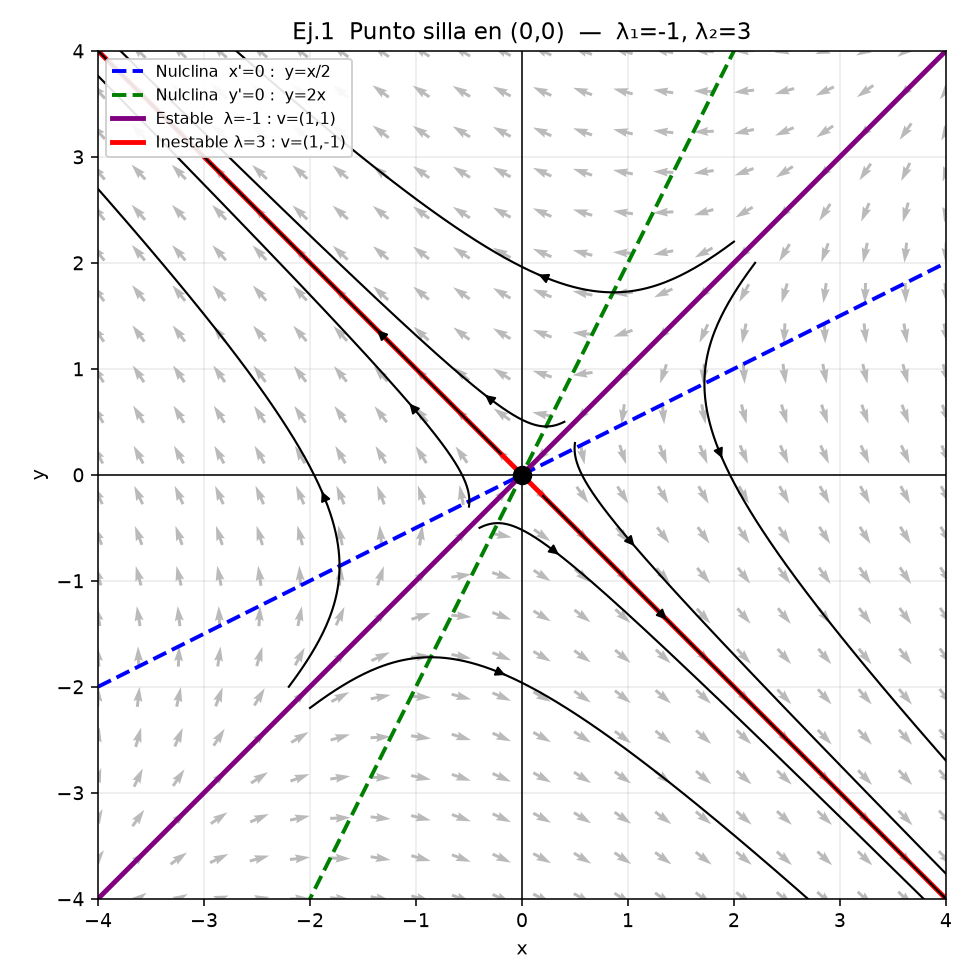
\includegraphics[width=0.55\textwidth]{ej1_silla.png}\end{figure}

%==================================================================
\seccion{Ejercicio 2 — Sistema NO lineal}

\[
\begin{cases}\dot x = x^2-y^2-1\\[2pt]\dot y = 2y\end{cases}
\]

\textbf{a) Nulclinas.}
\[
\dot x=0:\ x^2-y^2-1=0\Rightarrow \boxed{x^2-y^2=1}\ (\text{hipérbola, vértices }(\pm1,0));
\qquad
\dot y=0:\ \boxed{y=0}\ (\text{eje }x).
\]

\textbf{Puntos de equilibrio} (intersección). Con $y=0$: $\;x^2-1=0\Rightarrow x=\pm1$:
\[
\boxed{P_1=(1,0)}\qquad\text{y}\qquad\boxed{P_2=(-1,0)}.
\]

\textbf{Cómo corta el campo los ejes.}
\begin{itemize}
  \item Eje $x$ ($y=0$): $\dot x=x^2-1,\ \dot y=0$ (movimiento horizontal; el eje es invariante).
        Si $|x|>1\Rightarrow\dot x>0$ (se aleja); si $|x|<1\Rightarrow\dot x<0$ (hacia el centro).
  \item Eje $y$ ($x=0$): $\dot x=-y^2-1<0$ (siempre a la izquierda) y $\dot y=2y$:
        $\;y>0\Rightarrow\nwarrow$, $\;y<0\Rightarrow\swarrow$.
\end{itemize}

\textbf{b) Clasificación} con la matriz Jacobiana:
\[
J(x,y)=\begin{pmatrix}\dfrac{\partial\dot x}{\partial x} & \dfrac{\partial\dot x}{\partial y}\\[2mm]
\dfrac{\partial\dot y}{\partial x} & \dfrac{\partial\dot y}{\partial y}\end{pmatrix}
=\begin{pmatrix}2x & -2y\\ 0 & 2\end{pmatrix}.
\]

\[
J(1,0)=\begin{pmatrix}2&0\\0&2\end{pmatrix}\Rightarrow \lambda=2,2\ (>0)
\ \Rightarrow\ \boxed{P_1=(1,0)\ \text{NODO INESTABLE (fuente)}}.
\]
\[
J(-1,0)=\begin{pmatrix}-2&0\\0&2\end{pmatrix}\Rightarrow \lambda=-2,\,2\ (\text{signos opuestos})
\ \Rightarrow\ \boxed{P_2=(-1,0)\ \text{PUNTO SILLA}}.
\]

\textbf{Trayectorias.} La segunda ecuación se integra sola:
\[
\dot y=2y\ \Rightarrow\ y(t)=y_0\,e^{2t}.
\]
Salvo sobre el eje $x$ ($y_0=0$), toda trayectoria \emph{se aleja exponencialmente} del eje horizontal.

\begin{figure}[htbp]\centering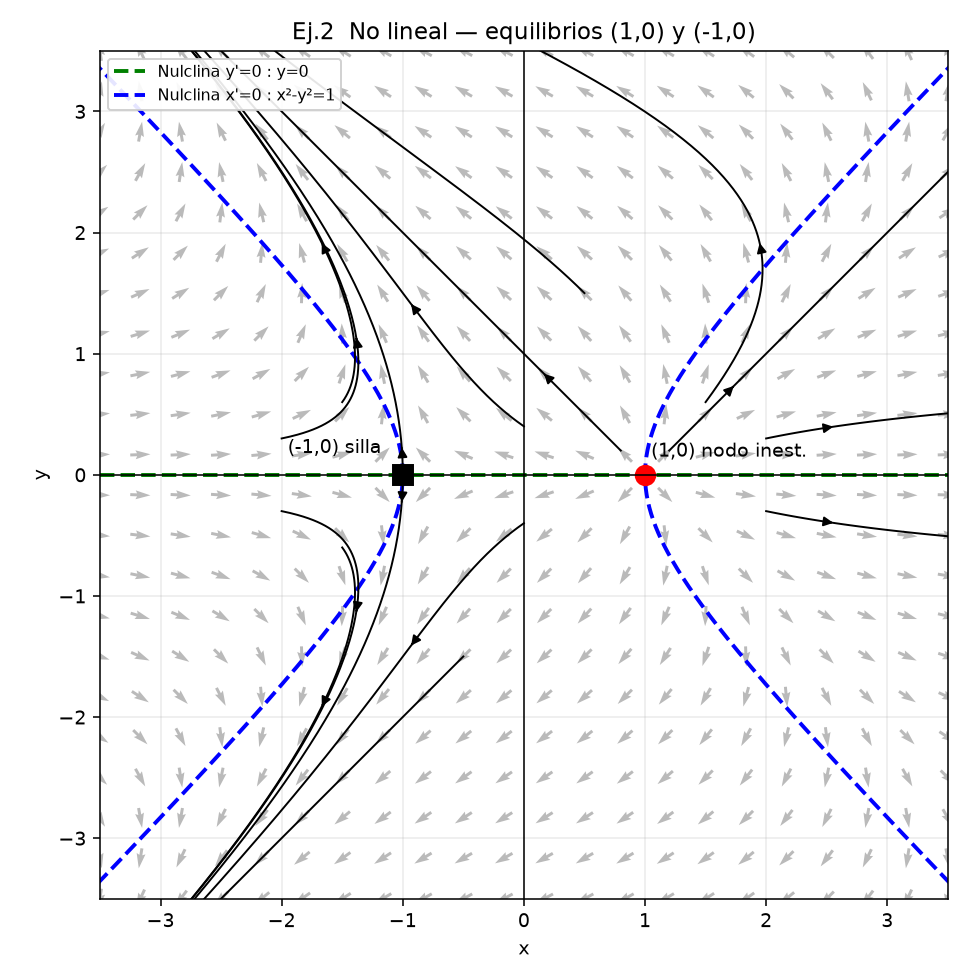
\includegraphics[width=0.55\textwidth]{ej2_nolineal.png}\end{figure}

%==================================================================
\seccion{Ejercicio 3 — Forma matricial: espiral estable}

\[
\dot{\vec x}=\begin{pmatrix} a & -2\\ 2 & 1\end{pmatrix}\vec x.
\]

\textbf{a) Valor de $a$.} Con traza y determinante:
\[
\operatorname{tr}=a+1,\qquad \det=(a)(1)-(-2)(2)=a+4,
\qquad
\lambda=\frac{\operatorname{tr}\pm\sqrt{\operatorname{tr}^2-4\det}}{2}.
\]

\emph{Condición 1 — espiral} (autovalores complejos): $\operatorname{tr}^2-4\det<0$.
\[
(a+1)^2-4(a+4)<0\Rightarrow a^2-2a-15<0\Rightarrow (a-5)(a+3)<0
\Rightarrow \boxed{-3<a<5}.
\]
\emph{Condición 2 — estable} (parte real $<0$): $\operatorname{tr}<0\Rightarrow a+1<0\Rightarrow \boxed{a<-1}$.

Intersección: $\boxed{-3<a<-1}$. \quad \textbf{Elijo $a=-2$:}
\[
\operatorname{tr}=-1,\ \det=2,\qquad
\lambda=\frac{-1\pm\sqrt{1-8}}{2}=\boxed{-\tfrac12\pm\tfrac{\sqrt7}{2}\,i}.
\]
Parte real $-\tfrac12<0$ y parte imaginaria $\neq0\Rightarrow$ \textbf{ESPIRAL ESTABLE} (converge al origen). $\checkmark$

\textbf{b) Sentido de giro.} En $(1,0)$: $\dot x=-2,\ \dot y=2\Rightarrow(-2,2)$ (arriba-izquierda)
$\Rightarrow$ giro \textbf{antihorario}, cerrándose hacia el origen.

\begin{figure}[htbp]\centering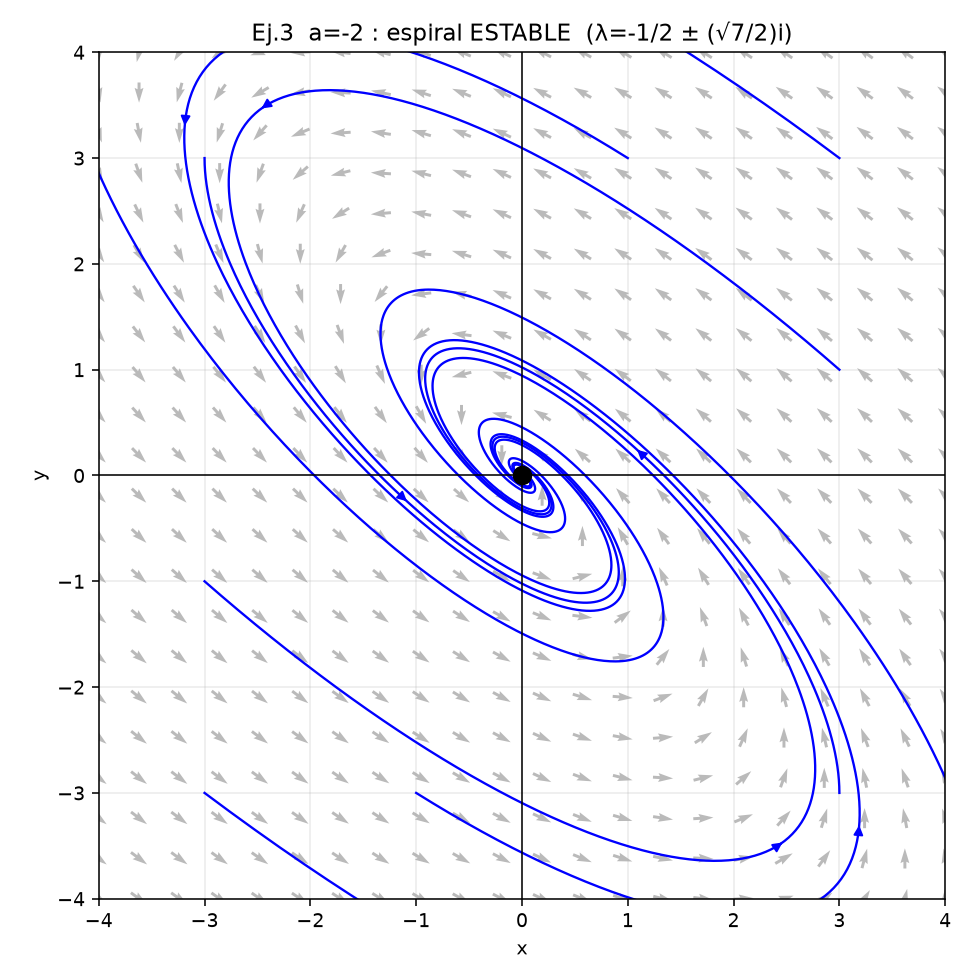
\includegraphics[width=0.55\textwidth]{ej3_espiral.png}\end{figure}

%==================================================================
\seccion{Ejercicio 4 — Modelo Romeo y Julieta}

\[
\begin{cases}\dot R=aR+bJ\\[2pt]\dot J=bR+aJ\end{cases}
\qquad
M=\begin{pmatrix} a & b\\ b & a\end{pmatrix}\ (\text{simétrica}).
\]

\textbf{Interpretación de los parámetros (según el enunciado).}
\begin{itemize}
  \item ``los sentimientos aumentan si el otro muestra interés'' $\Rightarrow$ término cruzado positivo: $\boxed{b>0}$.
  \item ``si siente que muestra demasiado interés se frena (no parecer desesperado)'' $\Rightarrow$ autoinhibición: $\boxed{a<0}$.
  \item ``amantes idénticos'' $\Rightarrow$ mismos $a,b$ (matriz simétrica).
\end{itemize}

\textbf{Equilibrio.} $\det(M)=a^2-b^2$. Si $a^2\neq b^2$, único equilibrio $(0,0)$ = indiferencia mutua.

\textbf{Autovalores y autovectores.} Para $\begin{pmatrix}a&b\\b&a\end{pmatrix}$:
\[
(a-\lambda)^2-b^2=0\Rightarrow a-\lambda=\pm b\Rightarrow
\boxed{\lambda_1=a+b\ \to\ (1,1)},\quad \boxed{\lambda_2=a-b\ \to\ (1,-1)}.
\]
$(1,1)$: $R,J$ del mismo signo (ambos aman o ambos odian). \quad
$(1,-1)$: signos opuestos (uno ama, otro odia).

\textbf{Análisis con $a<0,\ b>0$.} Siempre $\lambda_2=a-b<0$; el destino lo fija $\lambda_1=a+b$:

\begin{center}
\renewcommand{\arraystretch}{1.35}
\begin{tabular}{>{\bfseries}c l c c l}
\toprule
Caso & Condición & $\lambda_1=a+b$ & $\lambda_2=a-b$ & Tipo / destino\\
\midrule
1 & $b>|a|$ (cautela débil) & $>0$ & $<0$ & \textbf{Silla}: estalla a $\pm\infty$ según inicio\\
2 & $b<|a|$ (cautela fuerte) & $<0$ & $<0$ & \textbf{Nodo estable}: decae a $(0,0)$ (apatía)\\
3 & $b=|a|$ & $0$ & $<0$ & recta de equilibrios (caso límite)\\
\bottomrule
\end{tabular}
\end{center}

\textbf{Conclusión.} El caso interesante es la \emph{silla} (cuando la atracción $b$ supera la cautela $|a|$):
la componente sobre $(1,1)$ domina, así que si $R_0+J_0>0$ ambos sentimientos crecen
(\emph{amor mutuo}); si $R_0+J_0<0$ ambos caen (\emph{odio mutuo}).
La recta $J=-R$ (autovector estable) separa los dos destinos.

\textbf{Diagrama representativo} ($a=-1,\ b=2$): $\lambda_1=1>0$, $\lambda_2=-3<0\Rightarrow$ \textbf{punto silla}.

\begin{figure}[htbp]\centering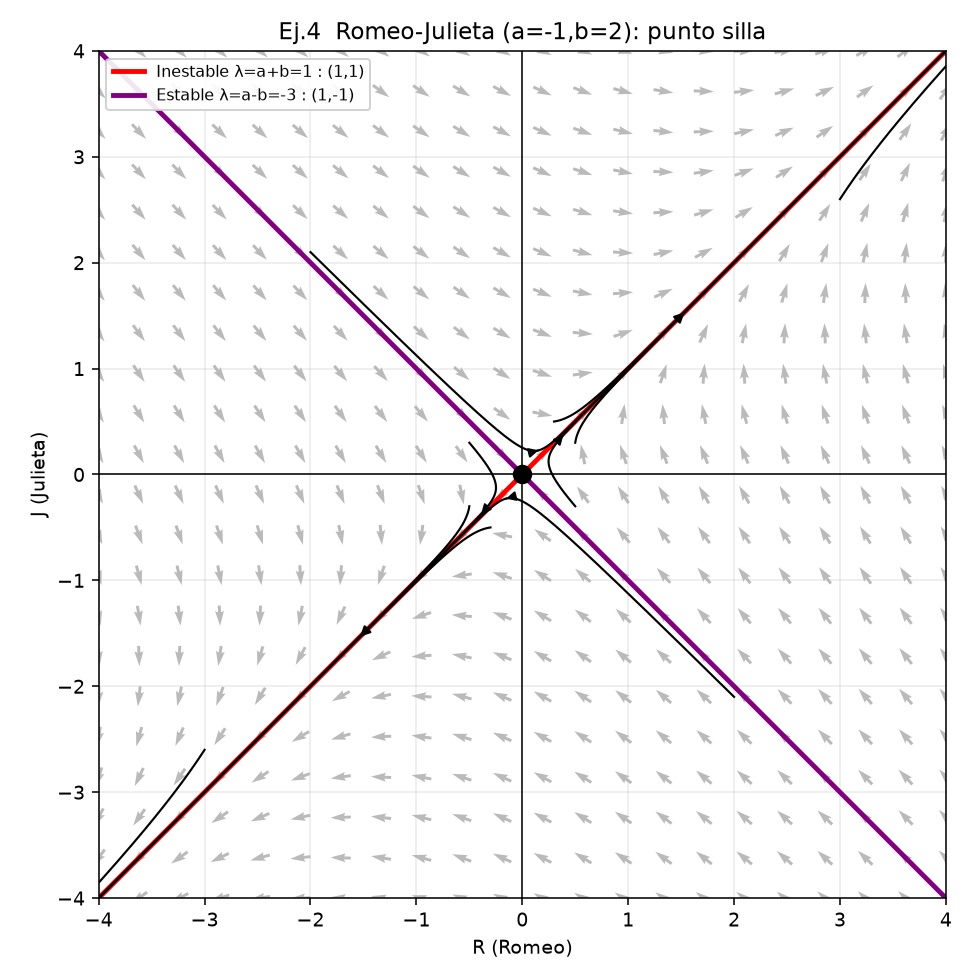
\includegraphics[width=0.55\textwidth]{ej4_romeo.png}\end{figure}

\vspace{4pt}
%==================================================================
\seccion{Resumen de clasificaciones}

\begin{center}
\renewcommand{\arraystretch}{1.35}
\begin{tabular}{c l l l l}
\toprule
Ej. & Sistema & Equilibrio(s) & Autovalores & Tipo\\
\midrule
1 & lineal & $(0,0)$ & $-1,\ 3$ & Punto silla\\
2 & no lineal & $(1,0)$ / $(-1,0)$ & $2,2$ / $-2,2$ & Nodo inestable / Silla\\
3 & $a=-2$ & $(0,0)$ & $-\tfrac12\pm\tfrac{\sqrt7}{2}i$ & Espiral estable\\
4 & $a<0,b>0$ & $(0,0)$ & $a+b,\ a-b$ & Silla o nodo estable\\
\bottomrule
\end{tabular}
\end{center}

\vspace{4pt}
\textbf{Truco general de clasificación:} calcular $\operatorname{tr}$ y $\det$.
\[
\det<0\Rightarrow\text{silla};\quad
\det>0,\ \operatorname{tr}^2-4\det>0\Rightarrow\text{nodo};\quad
\det>0,\ \operatorname{tr}^2-4\det<0\Rightarrow\text{espiral}.
\]
Y la traza define la estabilidad: $\operatorname{tr}<0$ estable, $\operatorname{tr}>0$ inestable.

\end{document}
